\section{22.01.24 : Snopki ($R$-modułów)}

  \buff{Presnopem} na kategorii $\mathbf{C}$ nazywamy dowolny funktor
  $$F:\mathbf{C}^{op}\to\mathbf{Set}$$

Snop na $X$ to presnop $F$, który dodatkowo spełnia:
\begin{align*}
  (\forall\;U\text{ otw w }X)(\forall\;U_\alpha\text{ otw. pok }U)(\forall\;s_\alpha\in F(U_\alpha))\\ 
  [(\forall\;\alpha,\beta\;)(s_\alpha\restriction_{U_\alpha\cap U_\beta}=s_\beta\restriction_{U_\alpha\cap U_\beta})\implies (\exists! s\in F(U))(\forall\;s\restriction_{U_\alpha}=s_\alpha)]
\end{align*}

\subsection{Usnopienie (sheafification)}
Niech $F$ będzie snopem na $X$. Źdźbło $F$ w $x\in X$ to 
$$F_x=\lim\limits_{\substack{\longrightarrow\\ U\ni x}}F(U).$$ Dla funkcji będzie to zgodność na pewnym otoczeniu $x\in X$. Dla $s\in F(U)$ i $x\in U$ oznaczamy przez $s_x$ obięcie $s$ w tej granicy - \emph{kiełek $s$ w $x$}.

Niech 
$$Et(F)=\bigsqcup_{x\in X} F_x$$ 
będzie przestrzenią z naturalnym rzutem 
$$\pi:Et(F)\to X$$ 
i topologią zadaną przez bazę 
$$\{\{s_x\;:\;x\in U\}\;:\;U\subseteq X, s\in F(U)\}.$$
Usnopienie $F$ to odwzorowania:
$$\overline{F}(U)=\{f:U\to Et(F)\;:\;f\text{ - ciągłe}, \pi\circ f=id_U\}.$$

\begin{center}
  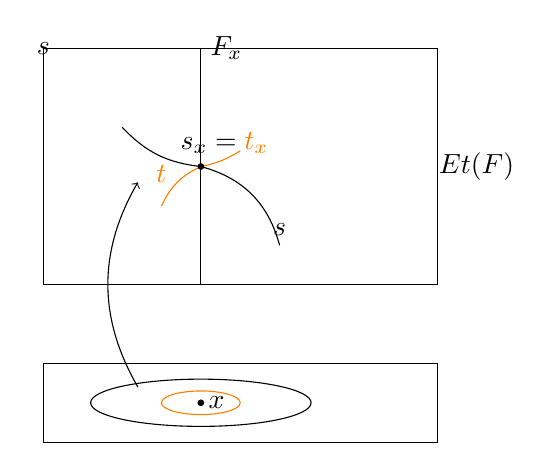
\begin{tikzpicture}
    \draw (0,0) rectangle (5, -3);

    \draw (0, -4) rectangle (5, -5);
    \draw (2, -4.5) circle (1.4 and 0.3);

    \draw (2, -3)--(2, 0) node [right] {$F_x$};
  \filldraw (2, -4.5) circle (1pt);
  \node at (2.2, -4.5) {$x$};
  \draw[orange] (2, -4.5) circle (0.5 and 0.15);

  \node at (5.5, -1.5) {$Et(F)$};

  \path (1, -1) edge [bend right=20] (2, -1.5);
  \path (2, -1.5) edge [bend left=30] (3, -2.5);

  \path[orange] (1.5, -2) edge [bend left=20] (2, -1.5);
  \path[orange] (2, -1.5) edge [bend right=10] (2.5, -1.3);

  \node at (3, -2.3) {$s$};
  \node at (1.5, -1.6) {$\color{orange}t$};

  \filldraw(2, -1.5) circle (1pt);
  \node at (2.3, -1.2) {$s_x=\color{orange}t_x$};

  \path[->] (1.2, -4.3) edge [bend left=30] (1.2,-1.7) node [midway] {$s$}; 
  \end{tikzpicture}
\end{center}

\begin{example}
  \item Presnop stały na $X$, czyli $U\mapsto \Z$, obcięcia to $id_{\Z}$. Wtedy przez usnopienie dostajemy snop lokalnie stały $U\mapsto \text{lokalnie stałe funkcje }U\to \Z$ i $Et=X\times \Z$. Oznaczam go $\Z_X$.
\end{example}

\begin{fact}
  \begin{enumerate}
    \item $\overline{F}$ jest snopem i $\overline{F}_x=F_x$ (podwójne usnopienie jest tym samym co pojedyncze ustopnienie).
    \item Jeśli $F$ jest snopem, to $\overline{F}=F$.
    \item $Hom_{Sh(X)}(\overline{F}, G)=Hom_{PSh(X)}(F, G)$, gdzie $F$ to presnop, a $G$ to snop. To oznacza, że usnopienie konstruuje pewien kanoniczny obiekt, a nie jeden ze 100 możliwych.
  \end{enumerate}
\end{fact}

\begin{proof}
  Ćwiczenie
\end{proof}

\subsection{Własności snopów i kategorii snopów}

\begin{fact}
  Niech $F, G$ to snopy na $X$, a $f,g:F\to G$. Wtedy
  \begin{enumerate}
    \item $f=g\iff (\forall\;x\in X)\;f_x=g_x$
    \item $f$ jest 1-1 (na każdym $U$) $\iff$ $f$ jest $1-1$ na każdym źdźble
    \item $f$ jest izomorfizmem $\iff$ jest izomorfizmem na każdym źdźble
  \end{enumerate}
\end{fact}

\begin{example}
\item Nie prawdą jest, że jeśli $f$ jest epimorfizmem na źdźbłach, to $f$ też jest epimorfizmem. Niech $X=\C\setminus\{0\}$. Mamy
  $$O_X\xrightarrow{\partial z} O_X$$
  i dla $U\subseteq \C\setminus\{0\}$ 
  \begin{center}\begin{tikzcd}[row sep=small]
    O(U)\arrow[r] & O(U)\\ 
    f\arrow[u, phantom, sloped, "\in"] \arrow[r] & f'\arrow[u, sloped, phantom, "\in"]
  \end{tikzcd}\end{center}
  to odwzorowanie jest epimorfizmem na źdźbłach. Ale jeśli popatrzymy na Cały obraz, to mamy funkcję $\frac{1}{z}$:
  \begin{center}\begin{tikzcd}[row sep=small]
    O(X)\arrow[r, "\partial_z"] & O(X)\\ 
    \log z\arrow[u, phantom, sloped, "\notin"] \arrow[r] & \frac{1}{z}\arrow[u, phantom, sloped, "\in"]
  \end{tikzcd}\end{center}
\end{example}

\begin{proof}
  \begin{enumerate}
    \item $\implies$ jest jasne

      $\impliedby$

      Niech $s\in F(U)$, $f_U(s), g_U(s)\in G(U)$. Dla każdego $x\in U$ mamy 
      $$f_U(s)_x=f_x(s_x)=g_x(s_x)=g_U(s)_x$$
      i ładnie to widać na obrazku wcześniej. Jeśli kiełki w każdym punkcie są te same, to cięcia snopa też są takie same.

    \item $\implies$ załóżmy, że na pewnym kiełku $f_x(s_x)=f_x(s'_x)$. Ale wtedy istnieje otoczenie $x\in V$ takie, że $f_V(s_V)=f_V(s'_V)$. Z tego, że $f_V$ jest $1-1$, wnioskujemy, że $s_V=s_V'$ i w takim razie $s_x=s_x'$.

      $\impliedby$ Powiedzmy, że mamy $s, s'\in F(U)$ i niech $f(s)=f(s')$. Chcemy wywnioskować, że $s=s'$. Skoro $f(s)=f(s')$, to muszą się zgadzać na snopach, czyli dla wszystkich $x\in U$ $f(s)_x=f(s')_x$, dalej $f_x(s_x)=f_x(s'_x)$. Z założenia $f_x$ jest $1-1$ na kiełkach, czyli $s_x=s'_x$ dla każdego $x\in U$, czyli $s=s'$.

    \item $\implies$ jest jasne

      $\impliedby$ Weźmy zbiór otwarty $U$ i mamy funkcję $f_U:F(U)\to G(U)$ która jest $1-1$ na mocy poprzedniego podpunktu. Pytamy, czy $f_U$ jest na?

      Niech $t\in G(U)$ będzie cięciem. Dla każdego $x\in U$ możemy znaleźć kiełek $s_x\in F_x$ taki, że $f_x(s_x)=t_x$. Skoro to się zgadza na kiełkach, to zgadza się też na otoczeniach, czyli mamy $V_x$ i $s_{V_x}\in F(V_x)$ takie, że $f_{V_x}(s_x)=t\restriction_{V_x}$.

      Skoro $f$ jest $1-1$, to kolekcja $(s_{V_x})_{x\in U}$ jest zgodna. Sklejamy ją do $s\in F(U)$ i $f(s)=t$.
  \end{enumerate}
\end{proof}

\begin{fact}
  \begin{enumerate}
    \item Presnopy grup abelowych tworzą kategorię abelową
    \item Snopy grup abelowych tworzą kategorię abelową
  \end{enumerate}
\end{fact}

Jądra w kategorii snopów zgadzają się z jądrami w kategorii presnopów, ale kojądra już niekoniecznie.

Kojądro w $Sh(X)$ (kategorii snopów gr. abelowych). Jeśli mamy $f:F\to G$, to 
$$(\ker f)(U)=\ker(F(U)\xrightarrow{f}G(U))$$
$$("\coker" f)(U)=\coker(F(U)\xrightarrow{f}G(U))$$
$"\coker" f$ zadaje presnop, ale niekoniecznie snop. Stąd prawdziwe kojądro to usnopienie tego fałszywca: $\coker f=\overline{"\coker"f}$.

\begin{center}\begin{tikzcd}
  F\arrow[r, "f"] & G\arrow[rr, "g"]\arrow[dr] & & H\\ 
                  & & "\coker" f \arrow[ur, "morf. pres." below, sloped, blue] \arrow[dr]\\ 
                  & & & \coker f\arrow[uu, "\exists", blue]
\end{tikzcd}\end{center}

Nie wiemy o jedyności tej strzałki w górę, ale jeśli spojrzymy na źdźbła, to wtenczas
\begin{center}\begin{tikzcd}
  G_x\arrow[rr]\arrow[dr, "epi" below, sloped] & & H_x\\ 
                & "\coker" f \arrow[dr, "\cong", sloped]\\ 
                &  &\coker f\arrow[uu]
\end{tikzcd}\end{center}

\begin{uwaga}
  Ciąg snopów $F\to G\to H$ jest dokładny w $Sh(X)$ $\iff$ dla każdego $x\in X$ $F_x\to G_x\to H_x$ jest dokładny.
\end{uwaga}

\begin{proof}Ćwiczenie\end{proof}

\begin{fact}
  W kategorii $Sh_R(X)$ snopów $R$-modułów nad $X$ jest dostatecznie dużo obiektów injektywnych.
\end{fact}

\begin{proof}
  Mamy snop $F$ i patrzę na jego źdźbło, które wkładam w pewien moduł injektywny $F_x\hookrightarrow I_x$. Definiujemy snop $I$ nad $X$:
  $$I(U)=\bigsqcap_{x\in U}I_x$$
  Niech $\iota_x$ będzie włożeniem $F_x$ w $I_x$. Wtedy $F(U)\ni s\mapsto (s_x)_{x\in U}\mapsto (\iota_x s_x)_{x\in U}\in I(U)$ i $\iota_x$ możemy skleić w $\iota:F\hookrightarrow I$.

  $I$ jest snopem injektywnym. Wtedy 
  \begin{center}\begin{tikzcd}
    )\arrow[r] & G\arrow[r]\arrow[d] & H\arrow[dl, dashed, blue]\\ 
               & I
  \end{tikzcd}\end{center}

  \begin{center}\begin{tikzcd}
    )\arrow[r] & G_x\arrow[r]\arrow[d, "g_x"] & H_x\arrow[dl, blue, "\exists\; \text{bo }I_x\text{ inj.}" below, sloped]\\ 
               & I_x
  \end{tikzcd}\end{center}

  \begin{center}\begin{tikzcd}
    O\arrow[r] & G(U)\arrow[r]\arrow[d] & H(U)\arrow[ddl, "\prod h_x", blue]\\
               & I(U)\arrow[d, sloped, phantom, "="]\\ 
               & \bigsqcap I_x
  \end{tikzcd}\end{center}
\end{proof}

\subsection{Flabby sheaf}

\begin{definition}[kohomologie snopa] 
  Funktor cięć globalnych $\Gamma:Sh_R(X)\to R-mod$ przypisuje
  $$\Gamma(F)=\Gamma(X, F):=F(X)$$
  Ten funktor jest lewo-dokładny i w związku z tym można patrzeć na jego wyższe funktory pochodne. To właśnie są jego kohomologie
  $$H^n(X, F):=R^n\Gamma(F)=R^n\Gamma(X, F).$$
\end{definition}

\begin{definition}
  Snop $F$ nad $X$ jest wiotki (flabby), jeśli dla każdego $U\subseteq X$ otwartego obcięcie $F(x)\to F(U)$ jest "na".
\end{definition}

Inaczej mówiąc, każda funkcja na otwarym podzbiorze rozszerza się na całe $X$.

\begin{theorem}
  \begin{enumerate}
    \item Każdy snop injektywny jest wiotki.
    \item Snopy wiotkie są $\Gamma$-acykliczne (czyli można ich używać do liczenia kohomologii)
  \end{enumerate}
\end{theorem}

\begin{proof}
  Zwiotczenie snopa buduje ze snopa $F$ snop $W(F)$ w który $F$ się włoży.

  \begin{definition}[zwiotczenie] 
    $$W(F)(U)=\prod_{x\in U}F_x$$
    "snop nieciągłych cięć $F$"
  \end{definition}

  \begin{enumerate}
    \item Niech $I$ będzie dowolnym snopem injektywnym. Możemy go włożyć w jego zwiotczenie 
      \begin{center}\begin{tikzcd}
        0\arrow[r] & I\arrow[d, "id"] \arrow[r, hookrightarrow] & W(I)\arrow[dl, blue, "r"]\\ 
                   & I
      \end{tikzcd}\end{center}
      niebieska strzałka jest z injektywności $I$.

      \begin{center}\begin{tikzcd}
        I(U)\arrow[d, "\bullet \restriction_U" left] & W(I)(U)\arrow[l, "r(X)" above]\arrow[d, "\bullet\restriction_U"]\\ 
        I(U) & W(I)(U)\arrow[l, "r(U)"]
      \end{tikzcd}\end{center}
      $\bullet\restriction_U$ jest "na", bo to snop wiotki. Czyli $r(X)$ jest "na" i tak samo $r(u)$. Wszystko dookoła $\bullet\restriction_U$ jest "na", czyli ono też takie jest.

    \item 
      \begin{enumerate}
        \item Jeśli $0\to F\to G\to H\to 0$ jest krótkim ciągiem dokładnym snopów, a $F$ jest wiotki, to wówczas odpowiedni ciąg cięć globalnych $0\to F(X)\to G(X)\to H(X)\to 0$  jest też dokładny.

          Trzeba sprawdzić $G(X)\to H(X)\to 0$. Niech $t\in H(X)$.

          Rozważamy pary $(U, s)$ takie, że $U$ jest otwarte w $X$, a $s\in G(U)$ jest cięciem takim, że $gs=t\restriction _U$. Być może nie wszędzie uda się tak podnieść, ale na pewno miejscami to zrobię, bo na źdźbłach też mamy dokładność.

          Zawieranie wraz ze zgodnością $s$ daje częściowy porządek, więc możemy użyć lematu Kuratowskiego-Zorna.

          Jeśli $(U, s)$ jest maksymalny, ale $x\in X\setminus U$, to powiększymy tego $s$.{\large\color{red}coś się zadziało}
      \end{enumerate}
  \end{enumerate}
\end{proof}
